
\chapter{AsthmaBuddy}
\label{chp:our-solution}

\section{Background}
In 2012, we did a similar project using Karotz \fnurl{Karotz}{www.karotz.com} as our platform\cite{CustomerDriven}. The thought behind Karotz is great. It is an open source robot which allows people to build applications and launch it to the Karotz store. However, in our subjective opinion, it is not ideal to work with. The Karotz starters kit costs ~\$200, not including customs, thus it is a pretty large investment for a family wanting to buy the product to use with our application. The API is only documented in French, which makes it a hassle, in addition to the fact that it is pretty cumbersome to configure for a ``non-technological'' family. 

\section{Technology}
We have looked around for other options than Karotz to create our tangible user interface, i.e. Arduino and Raspberry Pi. Arduino is an open source electronics prototyping platform\cite{arduino}, which allows for many different combinations of configurations, while \rpi{} is a cheap computer on the size of a credit card. Arduino shields comes in many shapes and sizes and is built for modularity and extendability. A wide-range of components are available if you want to add technical functionality to an Arduino system, such as Bluetooth, WiFi or small motors. 
While Arduino allows complex hardware configurations, Raspberry Pi makes larger abstractions, which seemed like the better choice for us as developers. Arduino programs are normally written in C\cite{strahl2000language}, and while there exists many tutorials and manuals for how to write Arduino code, we found the thought of writing in a programming language we had little prior knowledge of too challenging. Arduinos generally have low-powered CPUs, in order to keep them cheap. These low-powered CPUs tend to have problems with decoding MP3-files, which would lay constraints on our system. Due to these facts, we choose to develop the system on a Raspberry Pi.


\subsection{Raspberry Pi - Specifications overview}
The \rpi{} was initially intended to teach british school children about computer programming\cite{rasperrypi-about}. Since its release, it took an unexpected turn when lots of computer enthusiasts bought the product to do their own mini projects for a cheap price. 

The specification of a \rpi{} (Model B) is included in Table \ref{tab:pi-specs}. Figure \ref{fig:pi-arch-overview} shows an overview of the \rpi{}.        

\begin{table}[H]
\begin{tabular}{|p{6.0cm} | p{6.0cm} |}
\hline 
\textbf{Property} & \textbf{Specification} \\
\hline
CPU & 700 MHz ARM1176JZF-S core \\
\hline
Memory & 512 MB \\
\hline
USB 2.0 ports & 2 \\
\hline
Video Output & HDMI \\
\hline
Audio Output & 3.5 mm jack, in addition to ability to play sound through HDMI \\
\hline
Low-level Peripherals & 8 x GPIO (General Purpose Input/Output) \\
\hline
Power Source & 5 volt MicroUSB \\
\hline
Storage & SD card (available with preinstalled OS) \\
\hline
Network & 10/100 Mbps Ethernet.  \\
\hline
\end{tabular}
\caption{Raspberry Pi specifications}
\label{tab:pi-specs}
\end{table}

\begin{figure}[H] 
	\begin{minipage}[b]{0.4\linewidth}
	\centering
		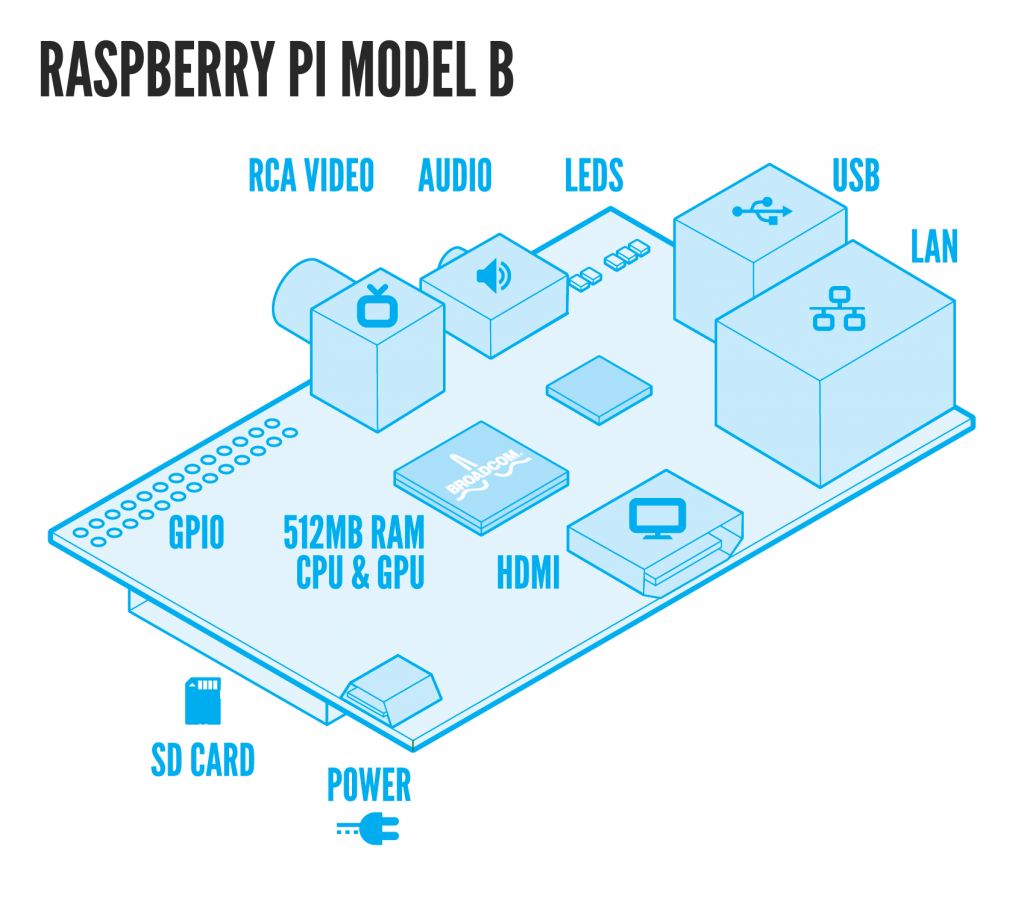
\includegraphics[width=0.3\paperwidth]{Pictures/rpi-arch-overview.png}
	\caption[Raspberry Pi Model B Architecture]{Raspberry Pi Model B architecture. \emph{Image source: http://raspberrypi.org/faqs} }
	\label{fig:pi-arch-overview}
	\end{minipage}
	\hspace{2.0cm}
	\begin{minipage}[b]{0.4\linewidth}
		\centering
			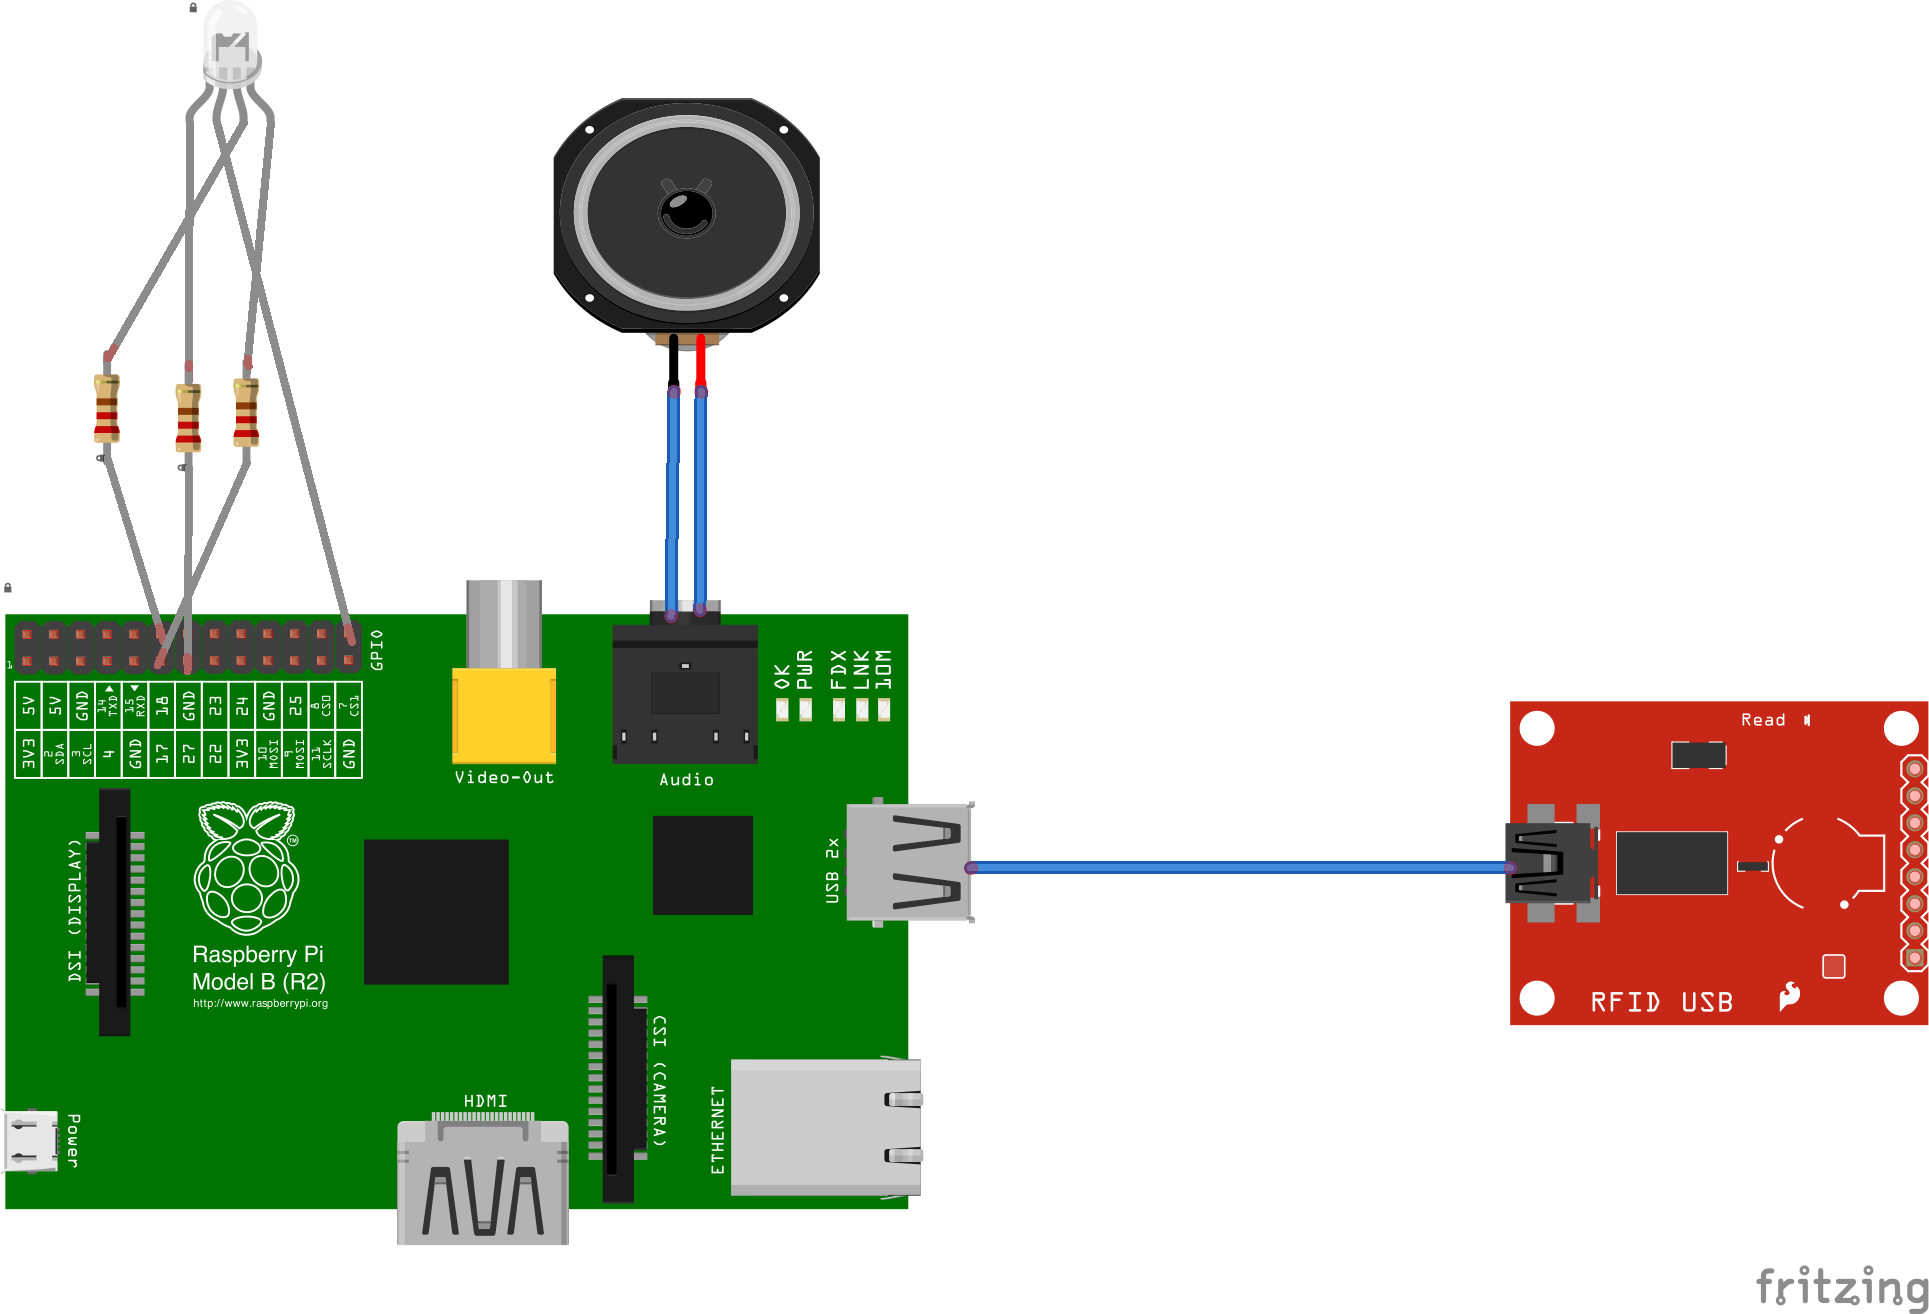
\includegraphics[width=0.3\paperwidth]{Pictures/pi-fritzing-model.png}
		\caption{Digital schematic over \rpi{} }
		\label{fig:pi-fritzing}
	\end{minipage}
\end{figure}
 
  
\subsection{Additional Components}
In addition to the \rpi{} we needed some components that children are able to interact through. These components and their functionality are summarized in this section. 


\paragraph{RFID Reader}
A child needs to be able to interact with AsthmaBuddy. We identified two approaches; using a button and/or using RFID technology to do it. We figured that having a big button on the top of a teddy bear would seem somewhat unnatural for a child. Additionally, this could cause problems with the wires inside the teddybear, as a child pushing a button could imply that AsthmaBuddy would be moved around. This could have been avoided by using a battery pack for the \rpi{}, but their capacity does not seem to exceed 24 hours when the \rpi{} is in idle mode. The conclusion was to use RFID technology to proceed in the medication process.


The RFID reader we used was a Sparkfun ID-12LA \fnurl{Sparkfun ID-12LA documentation}{http://tiny.cc/sparkfundoc}. One of the requirements of the USB reader was that it should be able to connect through an USB-port. 
         
\paragraph{USB speakers}
In order to play sounds to children, we decided to integrate speakers inside AsthmaBuddy. Since we did not want to pull too many wires out of the bear, we decided to use USB-powered speakers.    

\paragraph{LED lights}
We used LED lights connected to a breadboard in order to play around with the first prototype. The LED lights emits light in different colors to correspond to what action(s) is expected from the user during a treatment (see more in \ref{sec:proto1}).

\paragraph{Pi4j}
Pi4j\fnurl{Pi4j}{http://pi4j.com} is a Java framework that allows development for \rpi{} in Java, without having to write anything in C. 


Figure \ref{fig:pi-fritzing} shows a digital overview of \buddy{}. The green figure to the left is our \rpi{}. While it is also connected to a power supply and an internet cable, we chose not to include these in our figure. The red figure to the right is the RFID reader. It is connected to the \rpi{} through an USB cable. The black figure on top is the speaker, connected to the \rpi{} through the audio port. 
The grey lines and the lamp represents our LED light. It is connected to three of the GPIO (General Purpose I/O) ports on the \rpi{}, through a resistor. The last leg of the LED light is connected to ground on the \rpi{}, without a resistor.

\section{Design Rationale}
When designing \buddy{} we choose to use a teddy bear as an avator for our system. There are several reasons as to why we think this is an appropriate avatar. Teddy bears are well known toys, and has been loved for a long time. They are considered gender-neutral\cite{stagnitti1997determining}\cite{cherney2006gender} and in our subjective opinion it is a toy that could be discretely placed in a children's room. With the look of a teddy bear, \buddy{} can easily be placed among other toys and not be too visible. It was also important for us to choose a teddy bear of some size. A too thin bear could lead to problems with fitting the system inside the bear, and could in order lead to scepticism from the children. \buddy{} will bear resemblance to Tamagotchi\cite{tamagotchi} and Furby\cite{furby}, but \buddy{}'s purpose is to motivate, instruct and learn children about asthma, not being a toy meant purely for play. 

While designing our system we also wanted to make sure our system did not have robot-like features or robotic similarities. While children tend to find technology very interesting, we want to make \buddy{} seem as natural as possible, making a stuffed animal buddy, rather than a technological toy. We believe that these design choices serves our purpose of making children more aware of their asthma, while not being a constant reminder and a stress element.

Norwegian fire fighters have used a teddy bear in order to calm down children who find themselves in dramatic situations \fnurl{NRK: Firefighters use teddy bears to calm down children}{http://www.nrk.no/trondelag/bamser-i-utrykningsbilene-1.11548966}. The fire fighters state that the children respond positively to the teddy bear. 
While we were not able to find scientific research done on the use of teddy bears in dramatic situations, we found this news article interesting and a relevant mention to our research.

[Pictures of the bear we chose?]
 
 
\section{System Overview}
\label{sec:systemoverview}

\subsection{Use Cases}
Figure \ref{fig:pi-use-cases} shows a general overview of the use cases we have included in our prototype. A medication process can be started set off two ways:
A parent can register an alarm by using AsthmAPP. This alarm is then set of by the \code{AsthmaBuddy} instance running\footnote{The reader should take notice that the tangible user interface \ab{} differs from the program running on the \rpi{}, which is called \code{AsthmaBuddy}(note the change of font)}, giving the child a notification that it is time to take the relevant medicine.

The alternative to a registered alarm is if a child needs to take the medicine by need. In such case, the child or parent simply registers the RFID-tag before the child is guided through a quicker process (see Manuscript \ref{chp:anuscript}).  

\begin{figure}[H] 
	\centering
		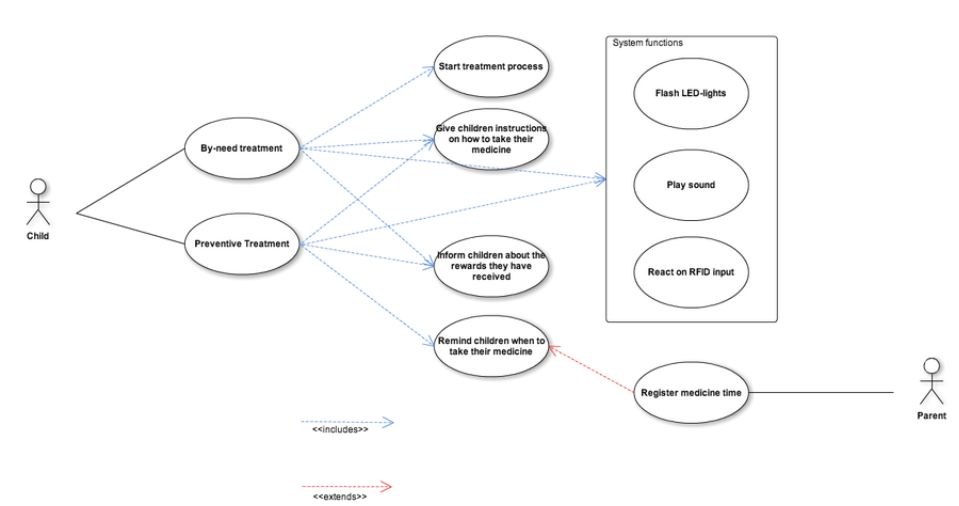
\includegraphics[width=0.8\paperwidth]{Pictures/usecases.png}
	\caption{AsthmaBuddy Use Cases}
	\label{fig:pi-use-cases}
\end{figure}

\subsection{Textual Use Cases}
\label{sec:textualusecasebyneed}

%--------- TEXTUAL USE CASE ----------
%--------- BY NEED TREATMENT ---------
\begin{table}[H]
\centering
\begin{tabular}{|p{4.0cm} | p{9.0cm} |}
\hline
\textbf{Title} & By need treatment \\
\hline
\textbf{Preconditions} & - \\
\hline 
\textbf{Scenario} & 
	\begin{enumerate}
	  \itemsep0em
	  \item User triggers treatment by holding a specific RFID-tag close to AsthmaBuddy.
	  \item System flashes LED-lights to notify user that the system is ready for use.
	  \item System plays sound to instruct the user to shake the medicine.
	  \item System plays sound to instruct user to mount the medicine on the mask and place the mask on his/her face.
	  \item User starts a treatment by interacting with AsthmaBuddy (by pressing it's hand or similar interaction).
	  \item System plays sound to count during treatment (1-2-3-4-5-6-7-8-9-10), while flashing lights for each count.
	  \item System plays sound to tell user he/she has done a good job.
	  \item System calculates reward based on health state.
	  \item System plays sound to award user with the calculated number of stars.
	  \item System plays sound to tell the user how many stars he/she has collected totally.
	\end{enumerate}
\\
\hline
	\textbf{Extensions} & 
		x.a User aborts treatment by not continuing the sequence.
\\
\hline
\end{tabular}
\caption{Textual use case: By need treatment}
\label{tab:textual-use-case}
\end{table}


%--------- PREVENTIVE TREATMENT -------

\begin{table}[H]
\centering
\begin{tabular}{|p{4.0cm} | p{9.0cm} |}
\hline
\textbf{Title} & Planned treatment \\
\hline
\textbf{Preconditions} & The current time corresponds with the time for a planned treatment. \\
\hline 
\textbf{Scenario} & 
	\begin{enumerate}
	  \itemsep0em
	  \item The system recognizes the time for a planned treatment.
	  \item The system starts blinking with LED-lights and playing sound to notify user.
	  \item Child interacts with AsthmaBuddy, to notify that he/she is ready for the treatment.
	  \item Start instructions by playing sound, telling the user to find a grown-up that can keep watch.
	  \item System waits for interaction to make sure the user is ready.
	  \item System tells the user to mount the medicine on the mask and put the medicine towards AsthmaBuddy's face.
	  \item System plays sound to simulate breathing.
	  \item System plays sound to tell the user how easy it was to take medicines and that it is the user's turn.
	  \item System plays sound to instruct user, telling the user to shake the medicine.
	  \item System waits for interaction to make sure the user is ready.
	  \item System plays sound to instruct user to put the mask on his/her face.
	  \item System plays sound counting to 10. 
	  \item System plays sound to tell the user he/she has done a good job.
	  \item System calculates reward based on health state.
	  \item System plays sound to award user with the calculated number of stars.
	  \item System makes a HTTPGet call to the server to find the total number of stars collected.
	  \item System plays sound to inform the user about how many stars the user has collected totally.
	\end{enumerate}
\\
\hline
	\textbf{Extensions} & 
		x.a Child does not interact with AsthmaBuddy when prompted
\\
\hline
\end{tabular}
\caption{Textual use case: By need treatment}
\label{tab:textual-use-case}
\end{table} 


\subsection{State Diagram}
\label{sec:statediagram}

In order to start the AsthmaBuddy application, we used SSH in order to gain access to the computer. We then retrieved the latest version of the source code from Git\fnurl{Git is the Source Code Management system we used}{http://git-scm.com/}, compiled it, and started running it (this process is described in Appendix \ref{app:asthmabuddy_manual}). Once AsthmaBuddy is running, it follows the state diagram depicted in Figure \ref{fig:asthmabuddy_statediagram}.  
  

\begin{figure}[H] 
	\centering
		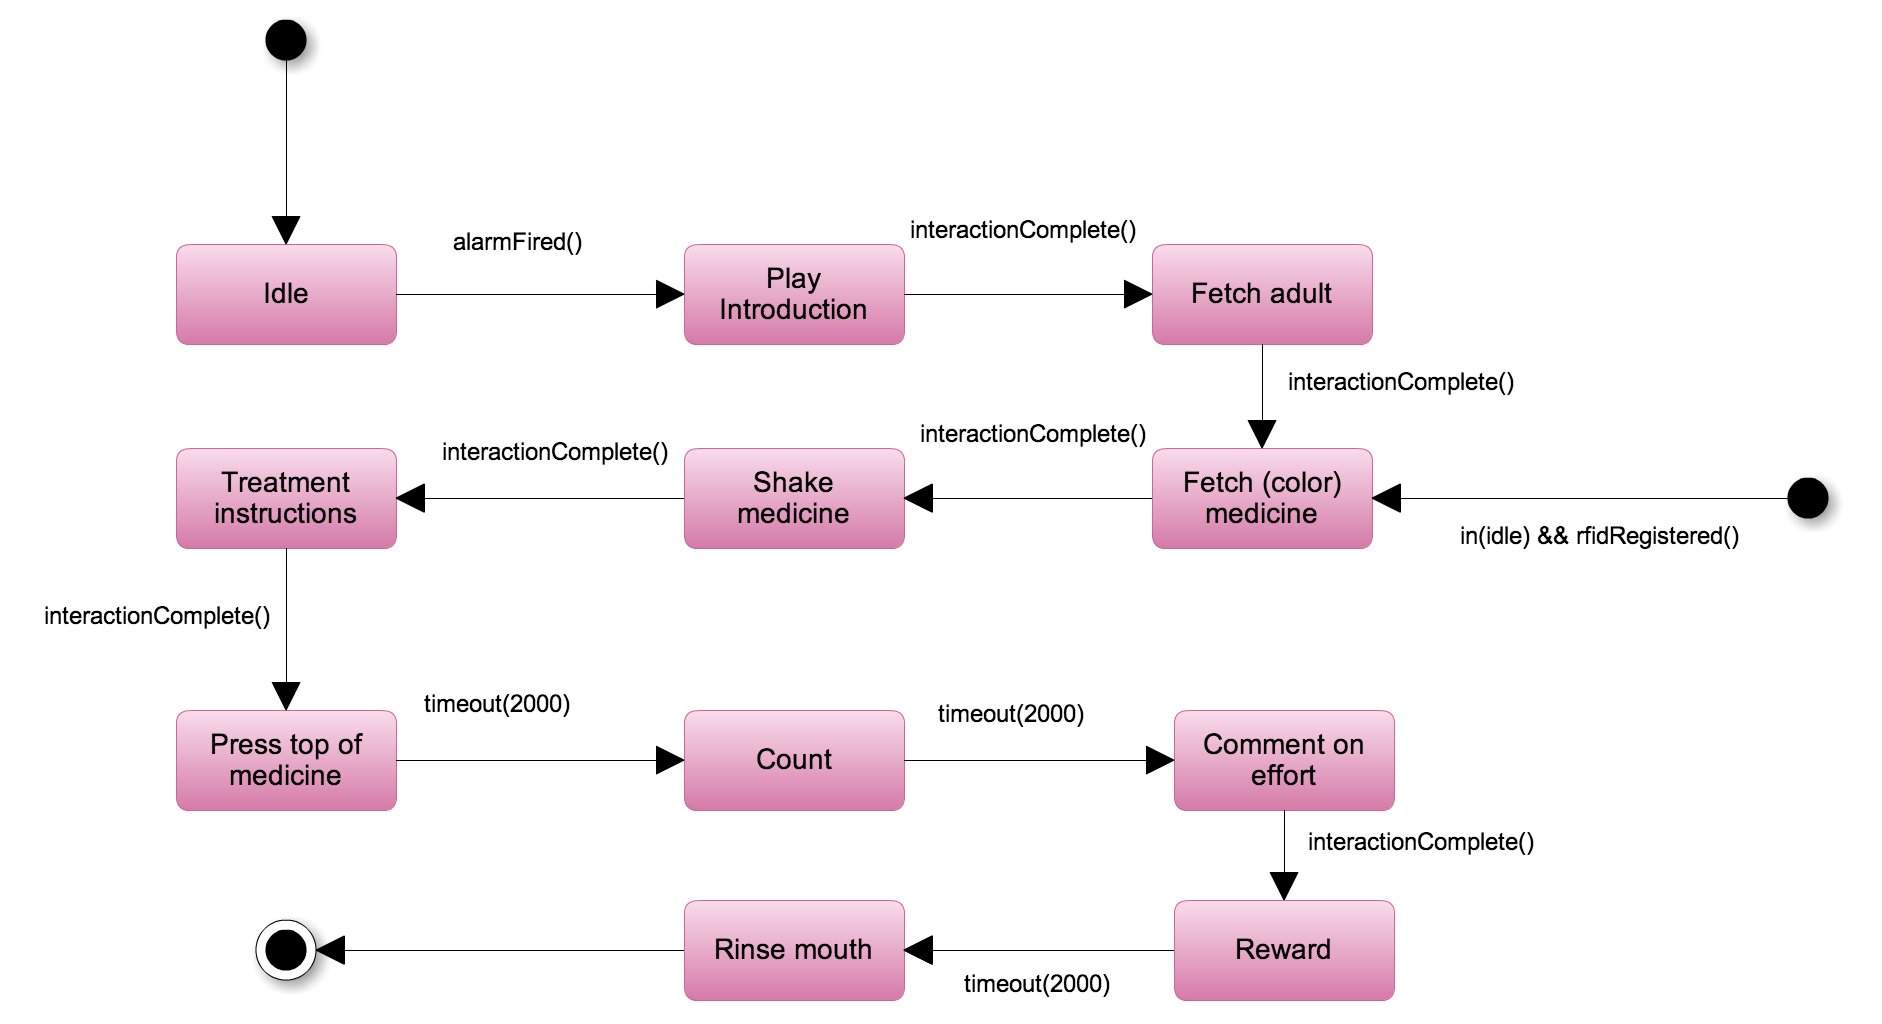
\includegraphics[width=0.7\paperwidth]{Pictures/statediagram.png}
	\caption{AsthmaBuddy State Diagram.}
	\label{fig:asthmabuddy_statediagram}
\end{figure}

\subsection{Sequence Diagram}
Figures \ref{fig:ab-sd-byneed} - \ref{fig:ab-sd-completing-treatment} shows sequence diagrams of how the system works internally. Some abstractions have been made, in order to reduce the cluster of arrows. 

\begin{sidewaysfigure}[htbp]
	\centering
		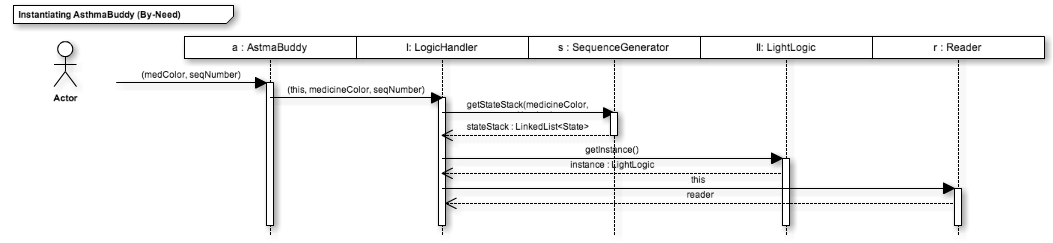
\includegraphics[scale=0.6]{Pictures/sd/sd-byneed.png}
	\caption{By Need Treatment - Sequence Diagram}
	\label{fig:ab-sd-byneed}
\end{sidewaysfigure}

\begin{sidewaysfigure}[htbp]
	\centering
		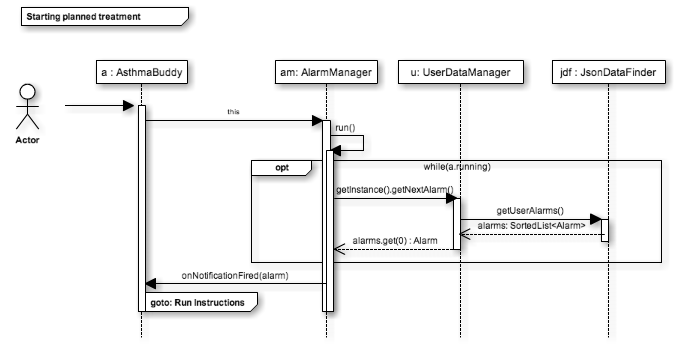
\includegraphics[scale=0.6]{Pictures/sd/sd-planned-treatment.png}
	\caption{Planned Treatment - Sequence Diagram}
	\label{fig:ab-sd-planned-treatment}
\end{sidewaysfigure}

\begin{sidewaysfigure}[htbp]
	\centering
		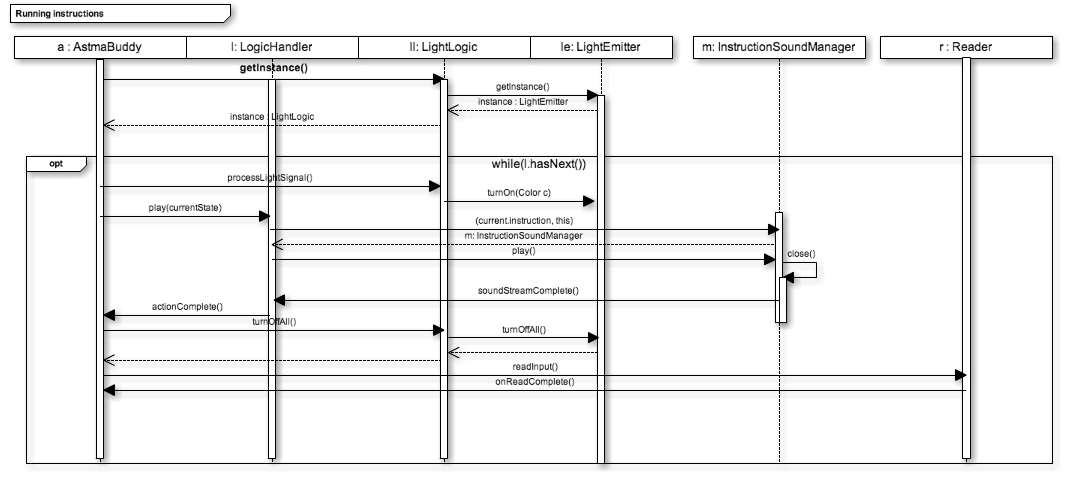
\includegraphics[scale=0.6]{Pictures/sd/sd-instructions.png}
	\caption{Playing Instructions - Sequence Diagram}
	\label{fig:ab-sd-instructions}
\end{sidewaysfigure}

\begin{sidewaysfigure}[htbp]
	\centering
		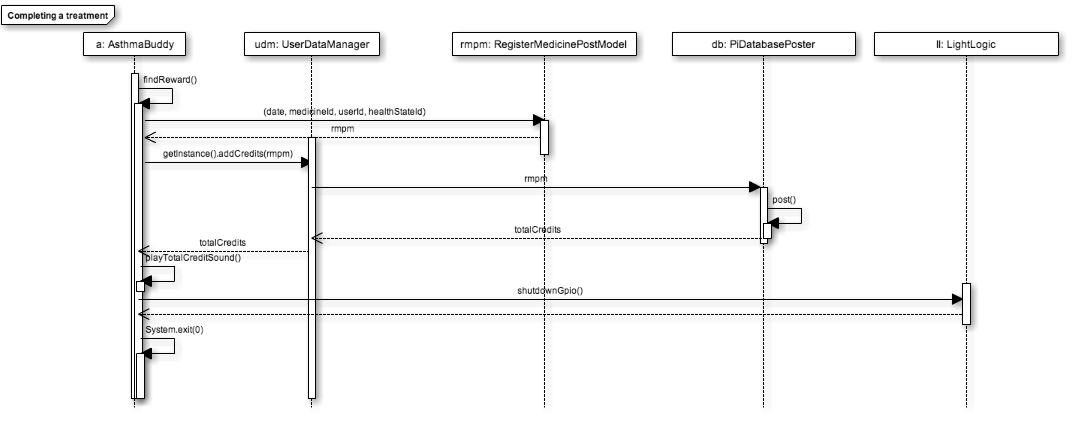
\includegraphics[scale=0.6]{Pictures/sd/sd-complete-treatment.png}
	\caption{Finishing a treatment - Sequence Diagram}
	\label{fig:ab-sd-completing-treatment}
\end{sidewaysfigure}


\begin{sidewaysfigure}[htbp]
	\centering
		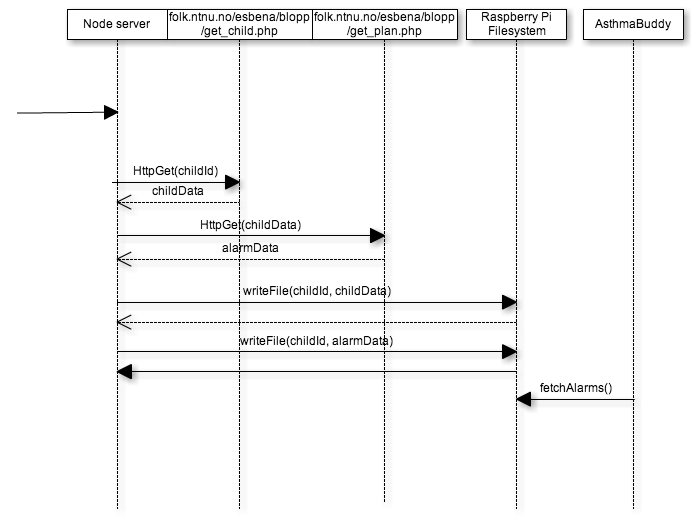
\includegraphics[scale=0.6]{Pictures/sd/sd-synchronizingv2.png}
	\caption{Synchronizing alarms - Sequence Diagram}
	\label{fig:ab-sd-synchronizing}
\end{sidewaysfigure}

\textbf{By Need Treatment}

We were not able to find a reasonable easy way to let the \buddy{} automatically be aware of the medicine that was to be taken at the start of a treatment. As a result, we used ssh into the \rpi{}, and provided the color of the medicine and the sequence number for the interaction that was to be tested.

After inserting these parameters, the \code{LogicHandler} retrieves a \code{LinkedList} of \code{Interaction}-objects that is to be played. After this sequence is ended, the system jumps to Figure \ref{fig:ab-sd-instructions}.
 
\textbf{Planned Treatment}

If an \code{AsthmaBuddy} instance is started without any parameters, it starts looking through alarm files (see Section \ref{sec:node-server}) every 60 seconds. If no alarm is returned from \code{UserDataManager}, it waits. Once an alarm is found, \code{AsthmaBuddy} is notified through \code{onNotificationFired}, which starts the treatment process. 
 
\textbf{Playing Instructions}

Playing instructions is mainly a loop of playing a sound, and turning on and off the LED-lights through the \code{LightEmitter} instance. 

\textbf{Finishing a Treatment}

When a treatment is finished, i.e. we are out of the \code{while} loop in Figure \ref{fig:ab-sd-instructions}, we register the treatment in the database. This ensures that the child is able to see the rewards in AsthmAPP. 


\subsection{Node Server}
\label{sec:node-server}
In addition to the Java application running on the \rpi{}, we developed a Node.js server\fnurl{Node.js}{http://nodejs.org/}. This backend system was developed in order to easily visualize the rewards given to a child after a treatment using \buddy{}. The initial problem is that AsthmAPP stores data to a MySQL database, with \code{childId} as the primary key for most tables. Initially, \buddy{} has no way of knowing which \code{childId} to add rewards to, or for which user alarms should be triggered. The current solution to our problem was to develop a Node.js server on AsthmaBuddy, which run as a background process. Whenever we want to switch users, AsthmAPP does an HTTP POST to this server, including the \code{childId} as a parameter. The server then retrives JSON-formatted data from our webservice, which includes the rewards a child has been given until now (for instance, by using a smartphone), and the alarms set for this user. 
When \buddy{} starts running, it checks for alarms to be set off every 60 seconds. When a child has finished a treatment, \code{AsthmaBuddy} updates the database, with the \code{childId} previously retrieved, and the number of stars a child collected during his/her treatment. With the data retrieved from the database, \buddy{} has the capability to tell the user how many stars a child has collected\footnote{Since this is a prototype, this functionality only works until a child has collected 20 stars. It became cumbersome to handle rewards totalling more than 20 stars}. This process is shown in Figure \ref{fig:ab-sd-synchronizing}.


 
\section{Prototype version 1}
\label{sec:proto1}
Our first prototype was a ``dumb'' version with the purpose of testing out different methods of interaction. We wanted to get as many different experiences as possible, in order to find what kids are thinking as ideal. Even though some of the interaction methods are infeasible to implement during the thesis, we wanted to know what children think of as fun interaction. We also found it important that children were motivated to give us honest results, so we wanted to give them freedom to be innovative and let their imagination play a part.  
%TODO: Skrive om
[TODO: Change to something useful, and actual\ldots] As a result, the first prototype was a simple state machine. The usability test was performed on NSEP's usability lab. Terje R\o sand sat in the backroom filming the sequence, while having a computer with ssh-connection to AsthmaBuddy. Whenever he observed that the children performed the method of interaction, he pressed enter in order for AsthmaBuddy to progress it's medication sequence. 

For the first prototype we tried out the following types of interaction with AsthmaBuddy:
\begin{enumerate}
	\item{Give AsthmaBuddy a ``High Five''}
	\item{Hold AsthmaBuddy's hand}
	\item{Hold smartphone close to AsthmaBuddy's belly}
	\item{Press AsthmaBuddy's nose}
	\item{Press \buddy{}'s belly}
	\item{Hold medicine close to AsthmaBuddy's mouth}
	\item{Hold RFID-chip close to \buddy{}'s nose}
	\item{Hold RFID-chip close to \buddy{}'s belly}
	\item{Clap your hands}
	\item{A variation of the above interactions}
\end{enumerate}

The prototype was not connected to the database. In order to show children their rewards, we simply added some stickers to a sheet of paper. 



\subsection{Information Gathering}

During the development phase we interviewed a couple of domain experts and parents in order to gather information about how they perform asthma treatments. 

\subsection{Evaluation of prototype version 1}

\paragraph{Evaluation of interaction methods}
\begin{table}[H]
\begin{tabular}{|p{5.0cm} | p{6.0cm} | p{3.0cm} |}
\hline 
\textbf{Interaction Method} & \textbf{Comments} & \textbf{Will it be in version 2?}\\
\hline
	Give AsthmaBuddy a ``High Five'' & & \\
\hline
	Hold AsthmaBuddy's hand & & \\
\hline
	Hold smartphone close to AsthmaBuddy's belly & & \\
\hline
	Press AsthmaBuddy's nose & & \\
\hline
	Press \buddy{}'s belly & & \\
\hline
	Hold medicine close to AsthmaBuddy's mouth & & \\
\hline
	Hold RFID-chip close to \buddy{}'s nose & The thickness of \buddy{}'s nose made it difficult for the RFID tag to communicate with our reader, this caused problems for the user. & No \\
\hline
	Hold RFID-chip close to \buddy{}'s belly & & \\
\hline
	Clap your hands & & \\
\hline
	A variation of the above interactions & & \\
\hline
\end{tabular}
\caption{Evaluation of interaction methods for AsthmaBuddy}
\label{tab:interactioneval}
\end{table}

\paragraph{Operating time}
The longest time for taking a planned treatment was about 2 minutes for an experienced user, and [XX] minutes for an inexperienced user. This treatment included the part where \buddy{} completes the treatment before the child. [SETT INN HVOR LANG TID DET TAR TIL VANLIG]. [SETT INN SAMMENLIGNING]. [VURDER OG KONKLUDER].     

A By Need treatment was registered to take about a minute for an experienced user. Usually, it takes approximately [XX] minutes to do a By Need treatment \footnote{Information gathered from parents}. [SETT INN SAMMENLIGNING]. [VURDER OG KONKLUDER].  

\paragraph{Feedback}
%Potential improvements
%New Interaction methods
%


\section{Prototype version 2}


\section{Further improvements}

 
%\subsection{Dealing with Bellotti's Challenges}
%\label{sec:handling-challenges}
%The main challenges Bellotti has identified (see Table \ref{tab:tuichallenges}) is \emph{``How to control or cancel system action in progress''} and \emph{``How to specify and select a possible object for action''}. We have previously stated that there are two cases in which a child will take their medicine, \emph{by need} and \emph{as a preventive measure}. An issue that could rise is how to detect when a child needs to take a medicine by need. Preventive medicines will fire alarms on AsthmaBuddy, and the child automatically knows that the system is ``awake''. However, when a child needs to take it by need, there is no other intuitive way to show that the AsthmaBuddy is awake than using LED-lights, which are the key for the system to work. Thus, the solution to the second challenge is usage of LED-lights. Cancelling operations, however, is difficult to find a ``good'' solution from a usability standpoint. 

%For instance, if AsthmaBuddy starts counting seconds on a treatment before a child is ready, there will be a need to reset this counter, or basically at any point during a treatment, go back to the last step. At the moment, the only solution we are able to see at this problem is to use RFID-chips to backtrack, modelling the treatment process as a statemachine. 
 